\subsection*{Coupled Cluster Doubles and Realistic Potentials}

In this section, we will perform CCD correlation energy calculations on a pure neutron matter system, using chiral potentials derived from effective field theory (EFT) to model the nuclear interaction. These potential more realistically models the nuclear interaction when compared to the Minnesota potential, so these results are expected to be more accurate than the Minnesota potential results from the previous section. Specifically, we use next-to-next-to-leading order (NNLO) chiral potentials in this section.

We will limit our calculations to a 66 neutron system for the chiral potential. This is done for two reasons. Ref. \cite{Ref8} and \cite{Ref9} show that, especially for pure neutron matter, calculations for a system of 66 neutrons are nearly indistinguishable from calculations performed at the infinite matter limit. So for 66 neutrons, the finite size error in a pure neutron matter calculation is minimized. Therefore, we do not need to perform extrapolations at higher values of N to perform an N$=\longrightarrow$ $\infty$ extrapolation.

Secondly, the CCD correlation energy calculations for pure neutron matter with chiral potential are very time intensive, much more so than pure neutron matter calculations with the Minnesota potential. For the Minnesota potential, the average time to generate converged CCD correlation energies across all densities in Figure \ref{pnm_mp_all} for 66 neutrons is 5.87 minutes. These calculations were all performed at 70 total energy shells or 6,142 single-particle states. However, when we perform the same calculations with the realistic chiral potentials from EFT, the average run time across all densities shown in Figure \ref{fig:ornl_pnm_ccd} is 2.32 hours per calculation. Moreover, these calculations converge at a much lower number of single-particle states, so these calculations were performed at 1,478 single-particle states or 27 total energy shells. Note that these calculations were performed with different codes, written in different languages, and performed with different high-performance computing set-ups. Hence, the run times are not directly comparable. However, it is sufficient to say that performing these calculations with realistic chiral potentials is much more computationally challenging than using the Minnesota potential.

As a further motivation for applying the SRE method to this system, let us examine the computational time and resources needed to perform calculations on a pure neutron matter system with 66 neutrons, a density of 0.16 fm$^{-3}$, and chiral NNLO potentials. Fig. \ref{fig:nnlo_ccd_times} shows the computational time in node seconds needed to perform the CCD correlation energy calculations as the number of single-particle states increases.

\begin{figure}
    \centering
    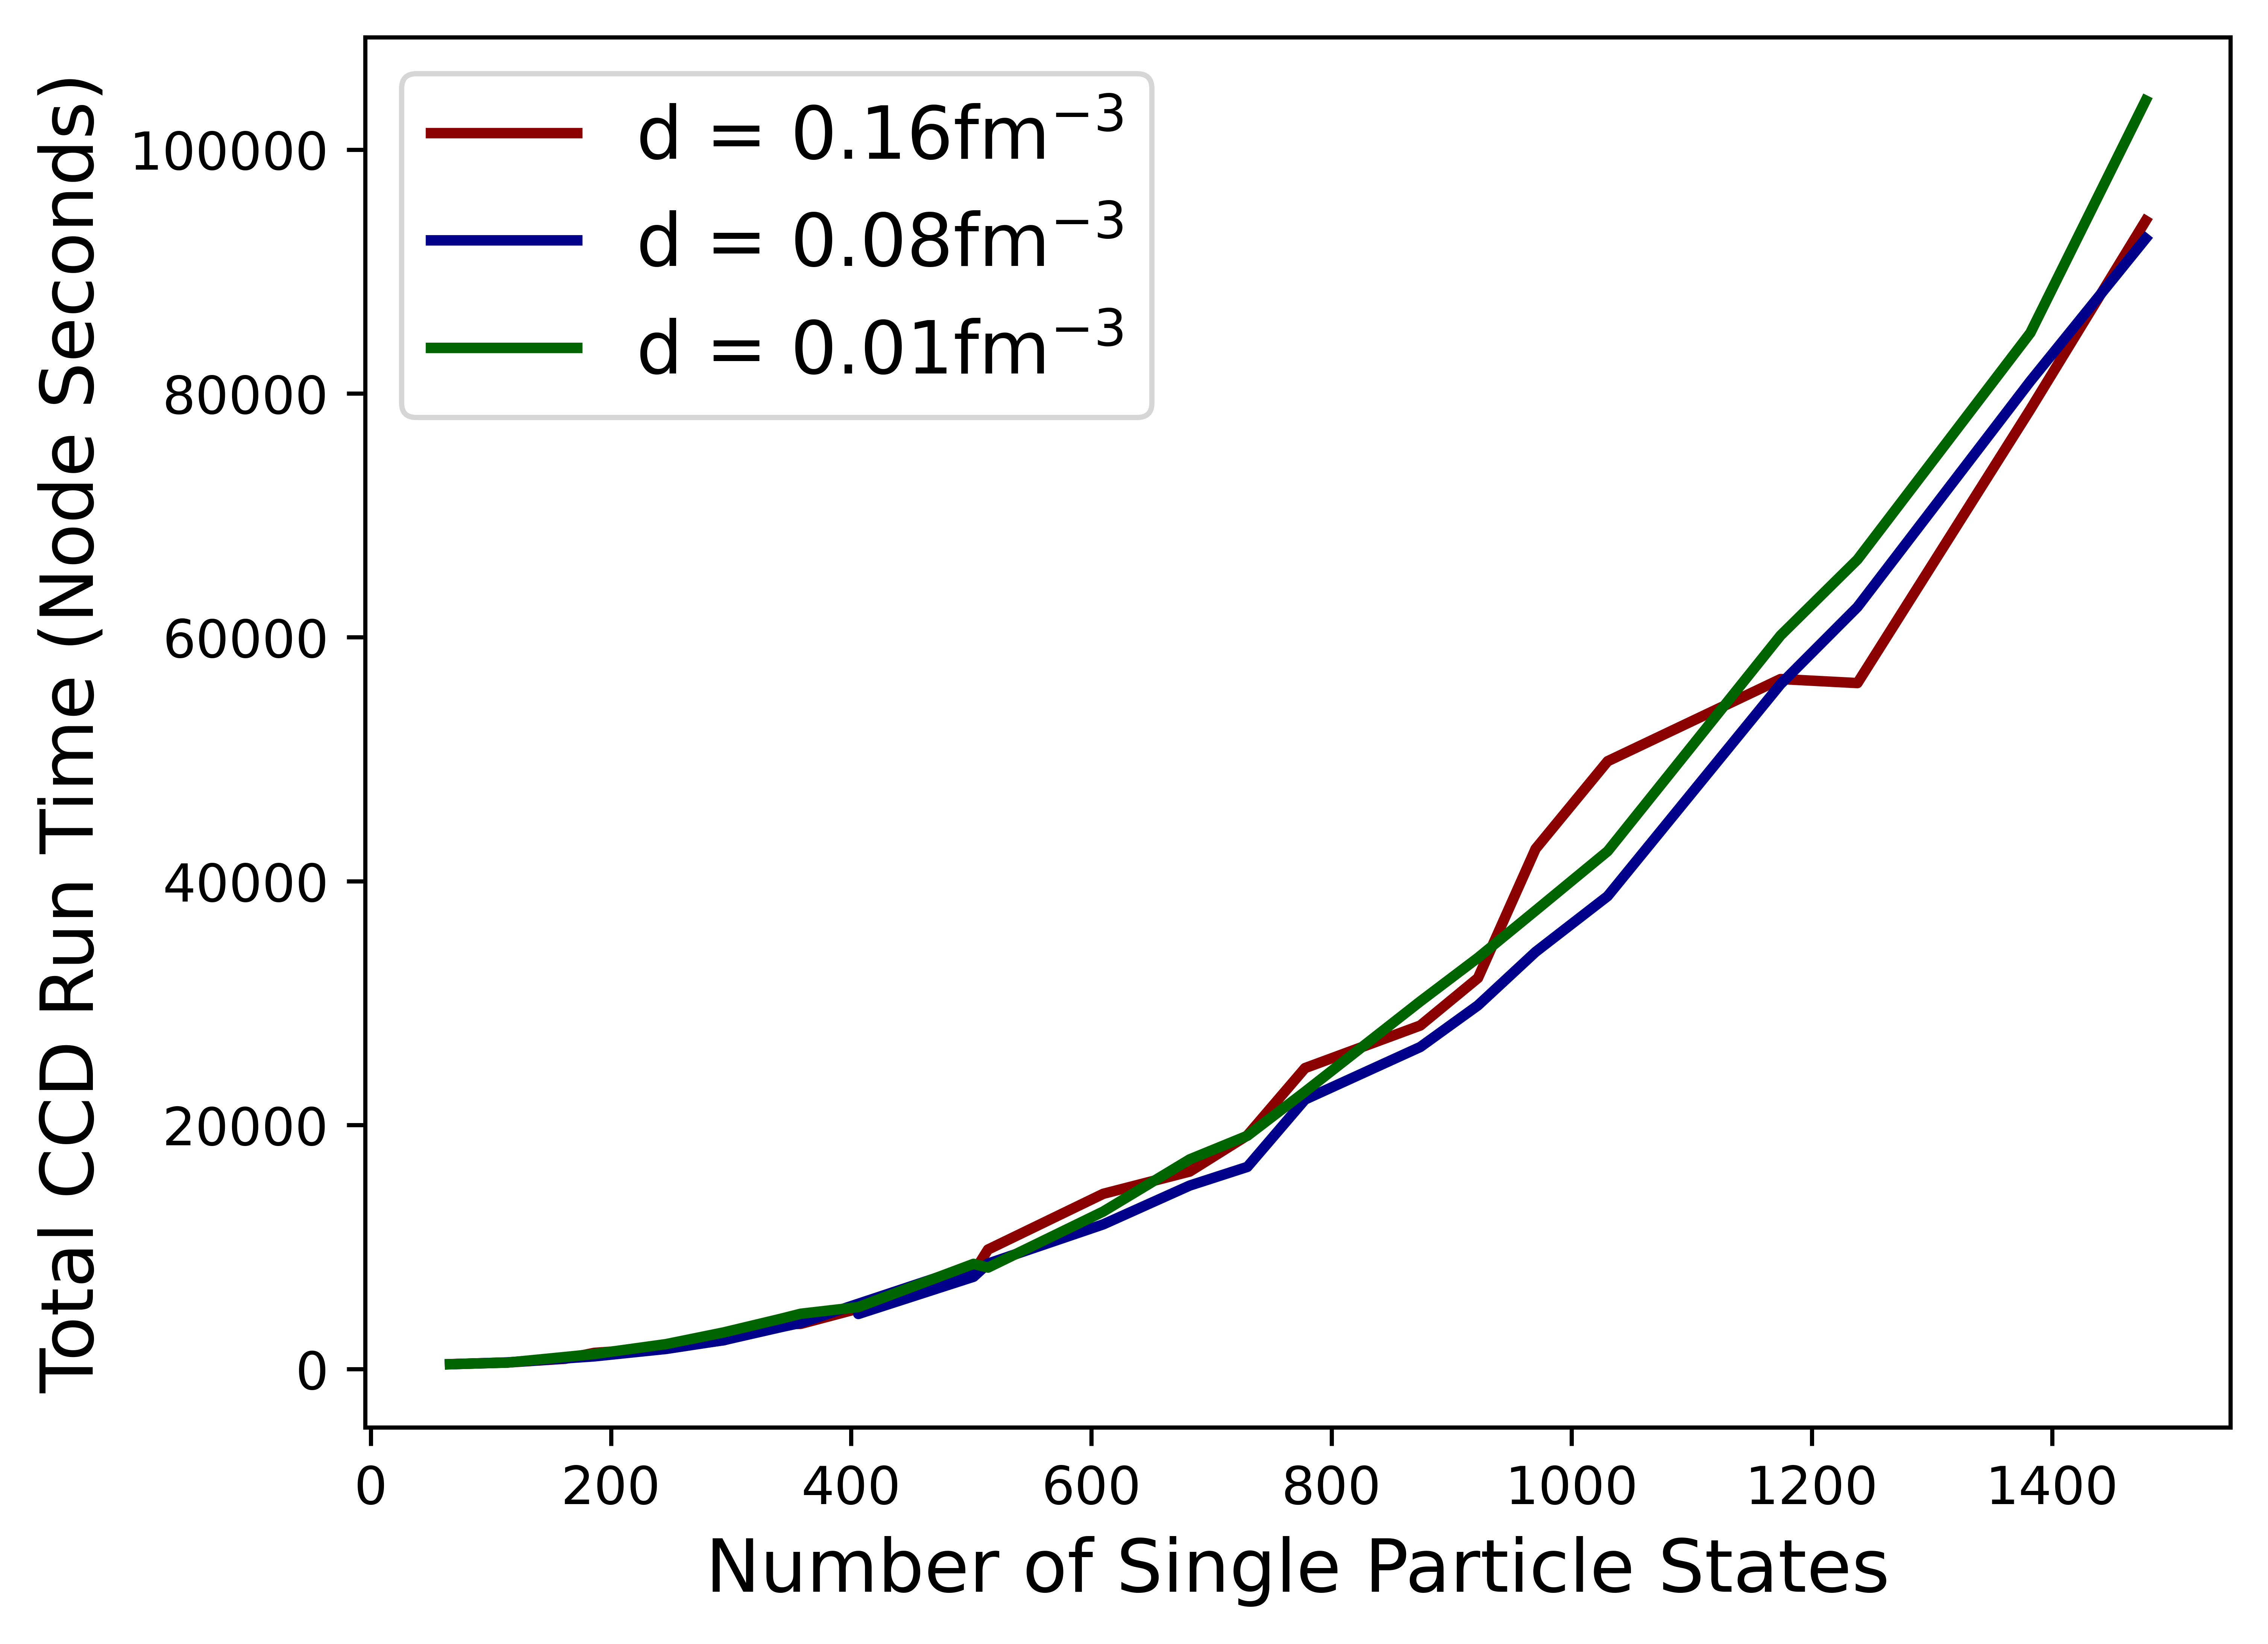
\includegraphics{Images/Chapter7/ORNL/pnm_times.png}
    \caption{Caption}
    \label{fig:nnlo_ccd_times}
\end{figure}


Figure \ref{fig:ornl_pnm_ccd} shows CCD calculations and ML predictions for pure neutron matter at 66 neutrons at two different density ranges. Figure \ref{fig:pnm_ccd_nuclear} shows a density range around nuclear density (which nuclear density being $\approx$ 0.16 fm$^{-3}$), and Figure \ref{fig:ornl_pnm_ccd_low} shows a low-density range. Densities around nuclear density are essential for studies of nuclei. The outer layers of a neutron star are thought to have densities around nuclear density (\cite{Ref3} \cite{Ref9} \cite{Ref16}), while the matter at the center of a neutron star is thought to be a low density (CITATION NEEDED). The ML specifications for the plots in Figure \ref{fig:ornl_pnm_ccd} are as follows. For \ref{fig:pnm_ccd_nuclear}, each ML prediction was made using only three training data points, MBPT2 and CCD correlation energy calculations between 114 and 186 single-particle states (or between 1 and 3 open shells). We were able to use such a small number of training points here because the correlation energies converge rather quickly. The SRE sequence length was chosen to be one here since there are only three training points. The converged CCD calculations in the figure were calculated at M=1,478 single particle states or 27 total energy shells (22 open energy shells). This number of single-particle states was chosen as the converged values because it is similar to the number of single-particle states used to calculate converged values in similar studies (Refs. \cite{Ref8}, \cite{Ref9}, and \cite{Ref20}). The same Gaussian Process algorithm and kernel as the Minnesota potential analysis was also used here, but the variance of the algorithm was chosen to be the standard deviation of the training data to the fourth power ($\alpha = \delta y_{train}^{4}$). For Figure \ref{fig:ornl_pnm_ccd_low}, the GP specifications are the same, but for the training data, seven training points were used from 186 to 502 single-particle states (3 to 9 open energy shells). This change was made because the correlation energy converges slower at lower densities. The SRE sequence length was also increased to three since more training data is available. The CCD correlation energy at M = 1,478 was still used at the fully converged value, though, and its convergence was confirmed.

\begin{figure}
\centering
\begin{subfigure}{.45\linewidth}
  \centering
  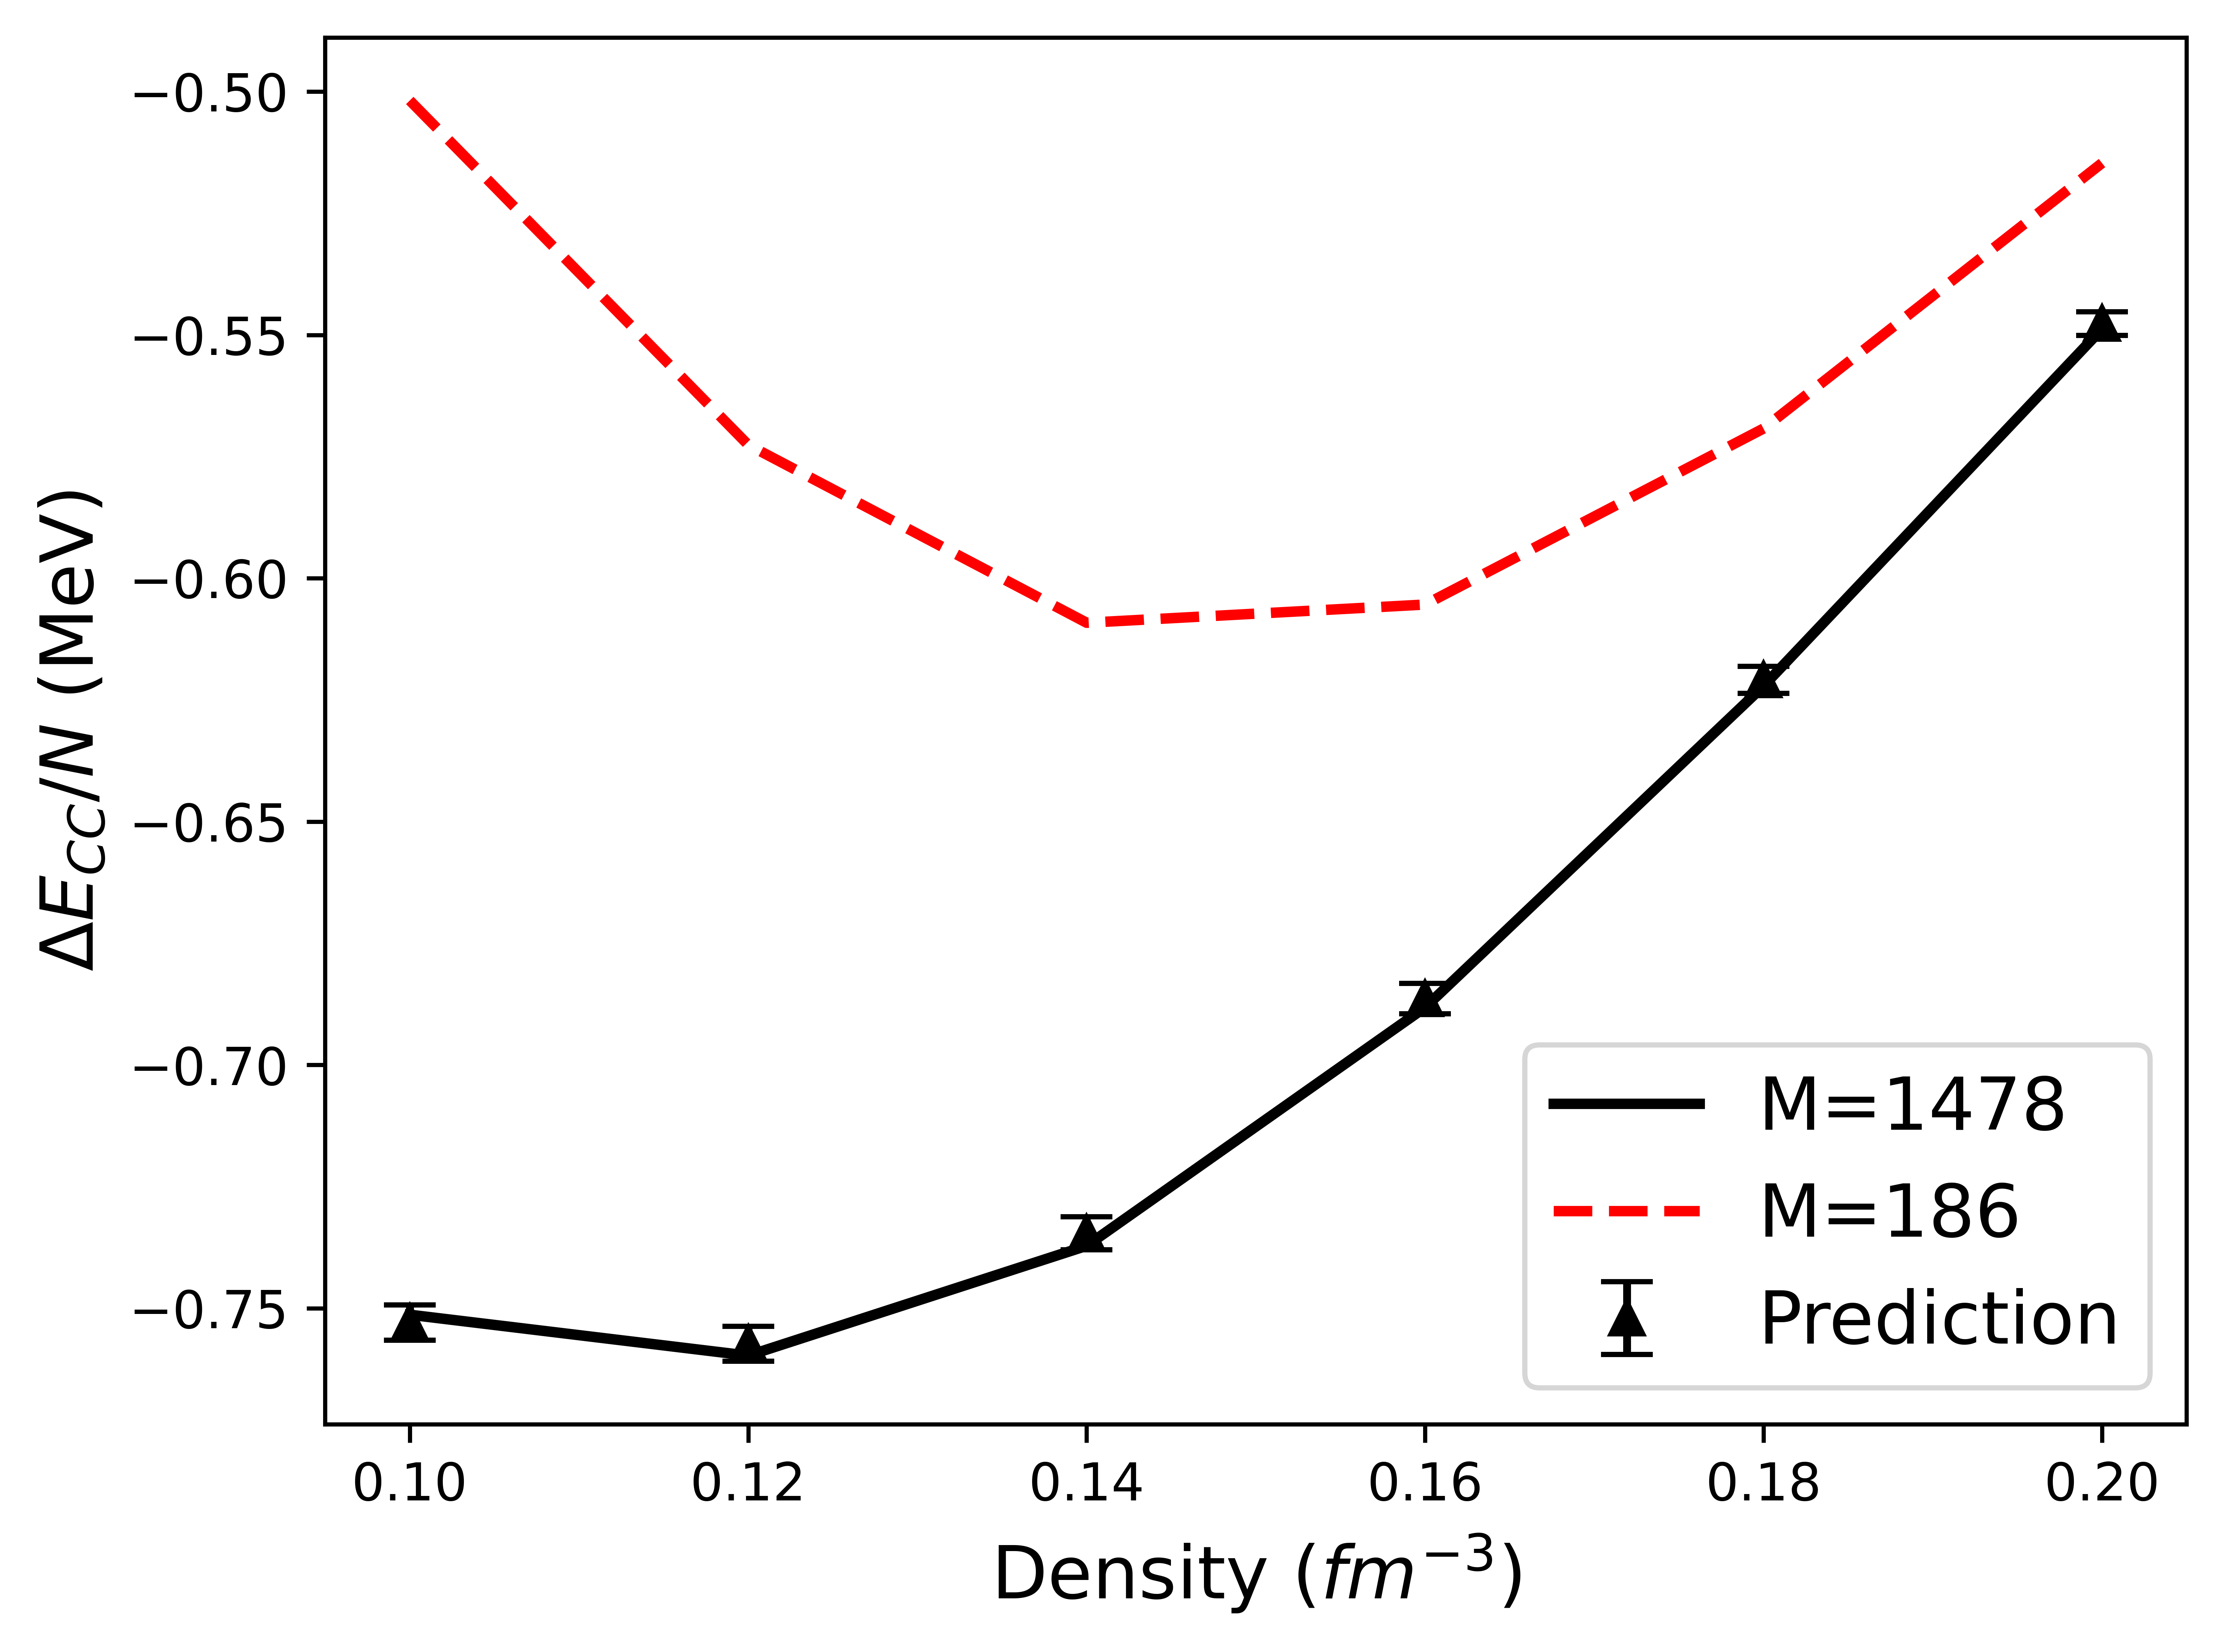
\includegraphics[scale=0.5]{Images/Chapter7/ORNL/neutron_matter-4.png}
  \caption{The results from predicting the converged $\Delta E_{CCD}/N$ for pure neutron matter at densities around nuclear density.  The average percent error across all densities is 0.25$\%$, and the time savings from generating only the training data versus the fully converged $\Delta E_{CCD}/N$ is 12.71 hours.}
  \label{fig:pnm_ccd_nuclear}
\end{subfigure}%
\begin{subfigure}{.45\linewidth}
  \centering
  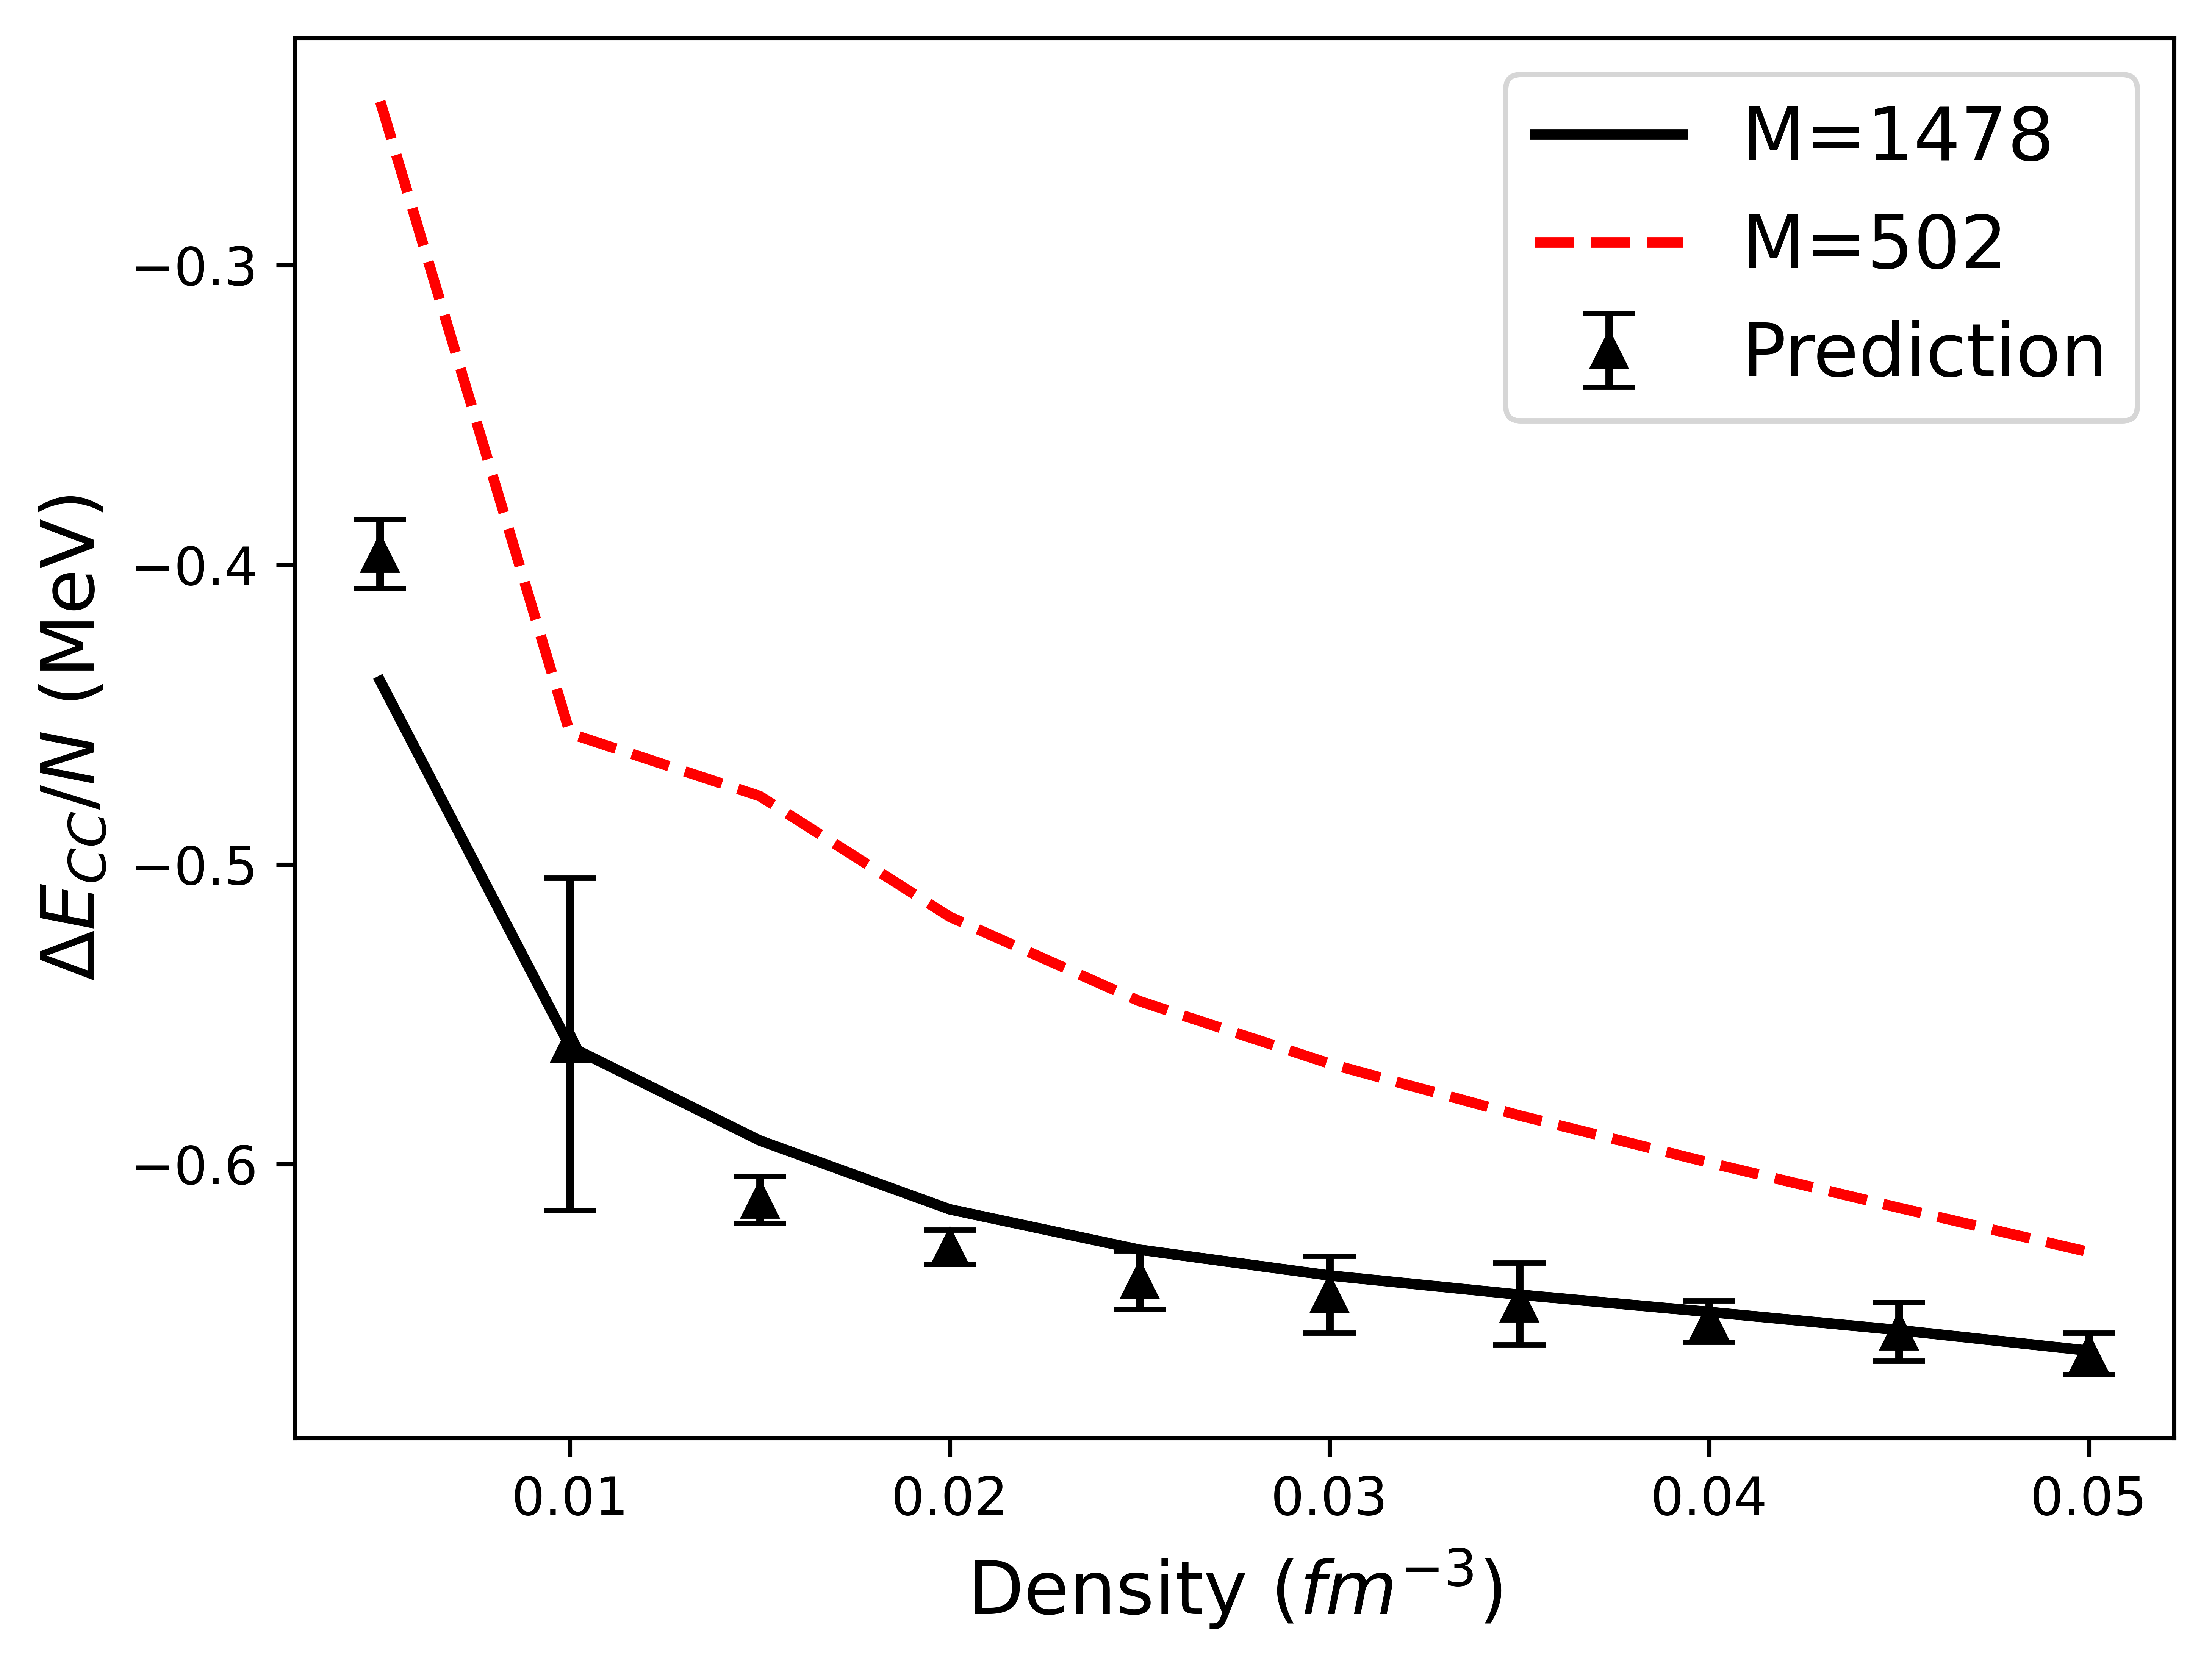
\includegraphics[scale=0.5]{Images/Chapter7/ORNL/neutron_matter_lowdensity-4.png}
  \caption{The results from predicting the converged $\Delta E_{CCD}/N$ for pure neutron matter at low densities.  The average percent error across all densities is 1.90$\%$, and the time savings from generating only the training data versus the fully converged $\Delta E_{CCD}/N$ is 18.27 hours.}
  \label{fig:ornl_pnm_ccd_low}
\end{subfigure}
\caption{The results from predicting the converged $\Delta E_{CC}/N$ for pure neutron matter using the coupled cluster doubles approximation.  Figure (a) shows pure neutron matter for a range of densities around nuclear density (0.10 $\leq$ d $\leq$ 0.20), and figure (b) shows the results for a low-density pure neutron matter (d $\leq$ 0.05). For both graphs, the solid black line plots the fully converged $\Delta E_{CCD}/N$, calculated at 1,478 single-particle states; the triangular markers represent the SRE predictions at each density of interest. The dashed red lines represent the point used to train the GP algorithms with the highest number of single-particle states (M = 186 for Fig. (a) and M = 502 for Fig. (b)) to show that the training set has not reached convergence.}
\label{fig:ornl_pnm_ccd}
\end{figure}

For Figure \ref{fig:pnm_ccd_nuclear}, the average percent error between the fully converged CCD correlation energies and the ML extrapolated CCD correlation energies is 0.25$\%$, and for Figure \ref{fig:ornl_pnm_ccd_low} it is 1.90$\%$. The slightly higher average percent error for the second figure is easily explained. The convergence of the correlation energy is slower at lower densities. Especially at d = 0.005 fm$^{-3}$ and d = 0.01 fm$^{-3}$, the correlation energies had not sufficiently converged at 1,478 single-particle states. This explains why there is a discrepancy between the ML prediction and the complete calculation at d = 0.005fm$^{-3}$. Additionally, the ML prediction at d = 0.01 fm$^{-3}$ closely matches the complete calculations, but there are pretty large error bars on the prediction when compared to the other predictions. This could also be explained by the slow convergence of the correlation energy at this point.

The timing data for \ref{fig:ornl_pnm_ccd} was collected using Michigan State University's high-performance computing center using Intel Xeon compute nodes running at 2.4 GHz and with 200GB of RAM each. For these calculations, 12 MPI nodes were used per calculation. For example, for Figure \ref{fig:pnm_ccd_nuclear}, generating the six fully converged CCD correlation energies at M = 1,478 single particle states took 13.03 hours. However, generating the training data for the six GP algorithms took only 0.32 hours, leading to a time savings of using the ML extrapolations of 12.71 hours. Additionally, for Figure \ref{fig:ornl_pnm_ccd_low}, it takes 24.16 hours to generate all ten fully converged CCD correlation energies and M = 1,478 single-particle states. However, it only takes 5.88 hours to generate the ten GP training data sets. Therefore using the ML extrapolation over doing the complete calculations saves 18.27 hours.

When considering both the accuracy and the time savings, the SRE method applied to CCD calculations of pure neutron matter with chiral potentials appears successful. The CCD correlation energies per particle can be accurately recreated for all but the smallest densities with very little training data and significant time savings.


\begin{figure}
    \centering
    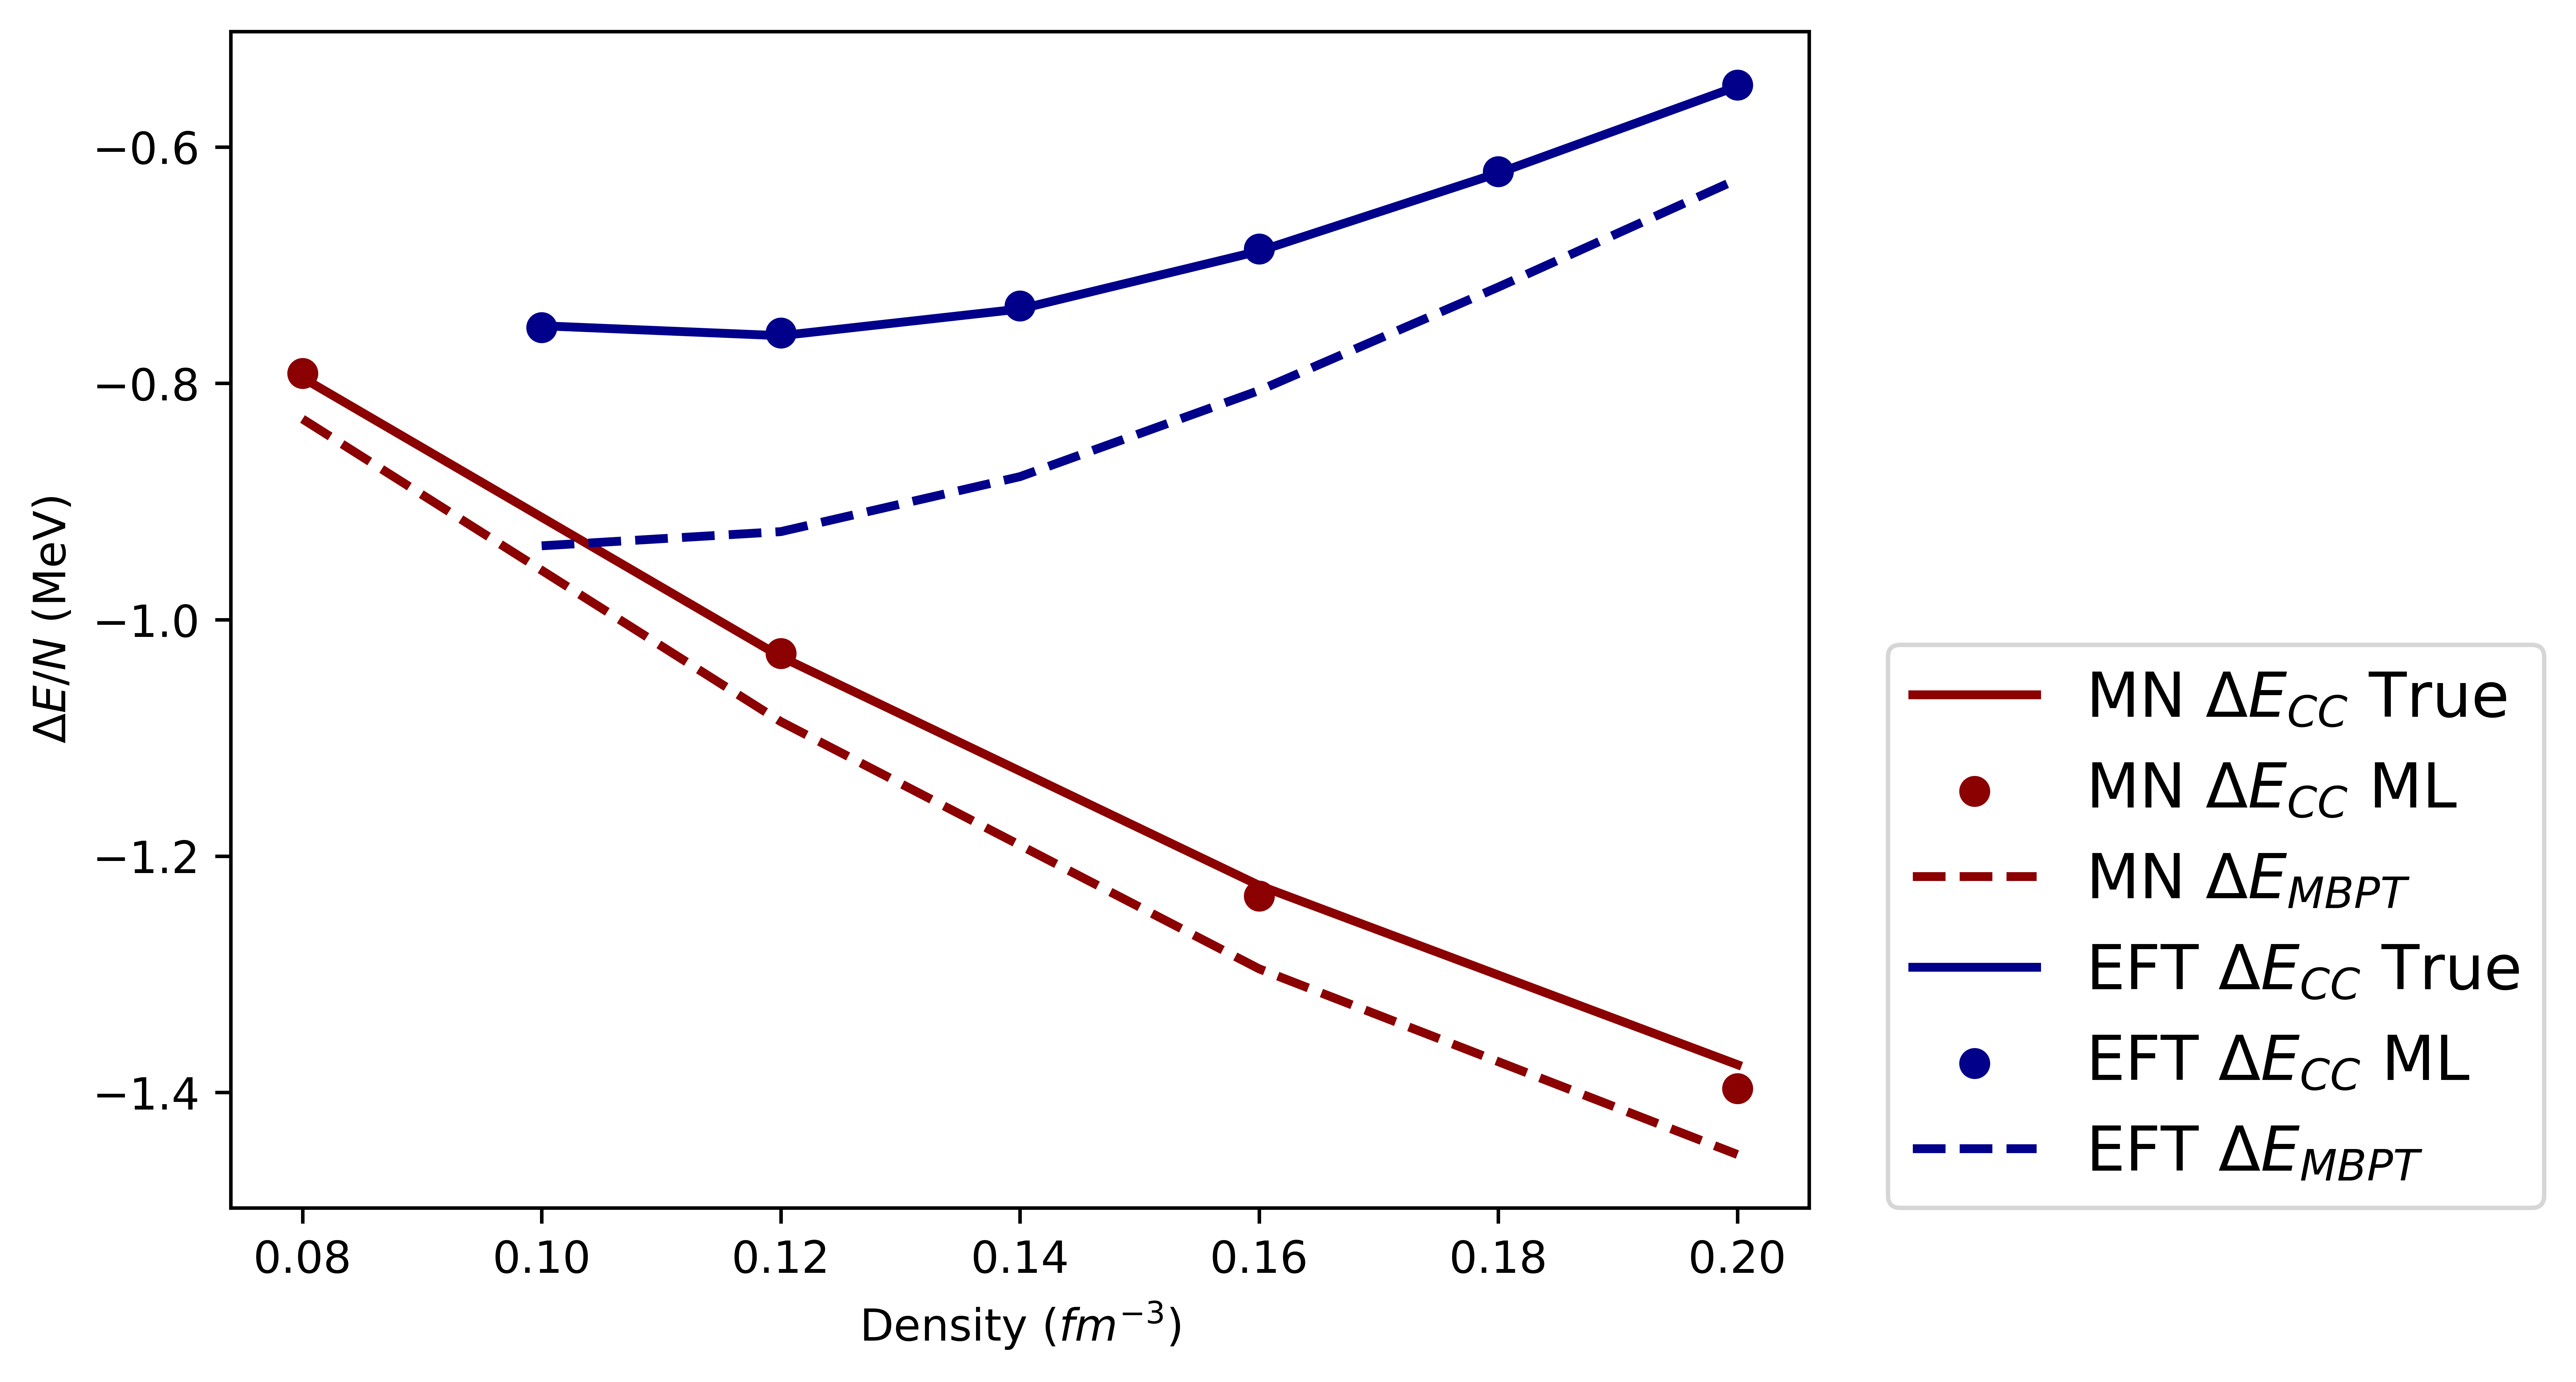
\includegraphics[scale=0.75]{Images/Chapter7/ORNL/EFT_and_MN.png}
    \caption{A comparison of correlation energy calculations for pure neutron matter near nuclear density for 66 neutrons.  The red data sets were calculated with the Minnesota potential, and the blue data sets with the chiral potentials. The dashed lines represent the converged correlation energy per particle from MBPT2, the solid lines represent the converged CCD correlation energies per particle, and the circular makers represent the ML predictions for the converged CCD correlation energies per particle.}
    \label{fig:eft_vs_mn}
\end{figure}

Figure \ref{fig:eft_vs_mn} compares pure neutron matter converged correlation energies per particle calculated with MBPT2 and CCD and for the Minnesota and chiral potentials. The Minnesota potential results are from calculations performed at 6,142 single-particle states of 70 total energy shells, and the chiral potential results are from 1,478 single-particle states or 27 energy shells. However, both the MBPT2 and CCD correlations energies have sufficiently converged. The ML predictions for the converged CCD correlation energy per particle are also shown. The results shown are for calculations involving 66 neutrons and near nuclear density. There are a few critical observations we can make from this graph. First, we know that the Minnesota and chiral potentials will produce different results as they model the nuclear interaction differently and to different levels of accuracy. The results differ significantly, with the chiral potentials yielding lower energy for both MBPT2 and CCD calculations.
Additionally, the difference in the results increases as density increases, indicating that there will be quite a significant difference between the two potentials at densities greater than nuclear density. Secondly, we can look at the difference between the MBPT2 and CCD results for the two potentials. For both potentials, the MBPT2 correlation energy per particle is lower than the CCD correlation energy per particle. However, for the Minnesota potential, the MBPT2 correlation energies are only slightly below the CCD correlation energies, and the gap between the MBPT2 correlation energies and the CCD correlation energies is roughly consistent over the entire density range shown. There is a more significant discrepancy between the MBPT2 and CCD correlation energies for the chiral potential, and this gap grows as the density decreases. Finally, it is essential to note that for each potential, the ML predictions to the converged CCD correlations energies are in good agreement with the total calculations, so the SRE method is potential independent.
